%%%%%%%%%%%%%%%%%%%%%%%%%%%%%%%%%%%%%%%%%%%%%%%%%%%%%%%%%%%%%%%%%%%%%%%%%%%

\documentclass{standalone}

\usepackage{amsmath}
\usepackage{mathptmx}
\usepackage{pgfplots}
\usetikzlibrary{external}
\tikzexternalize{yeast-error}
\pgfplotsset{compat=1.16}

%% IEEE uses Times Roman font, so we'll default to Times.
%% These three commands make up the entire times.sty package.
\renewcommand{\rmdefault}{ptm}
\renewcommand{\ttdefault}{pcr}
\normalfont\selectfont

\begin{document}

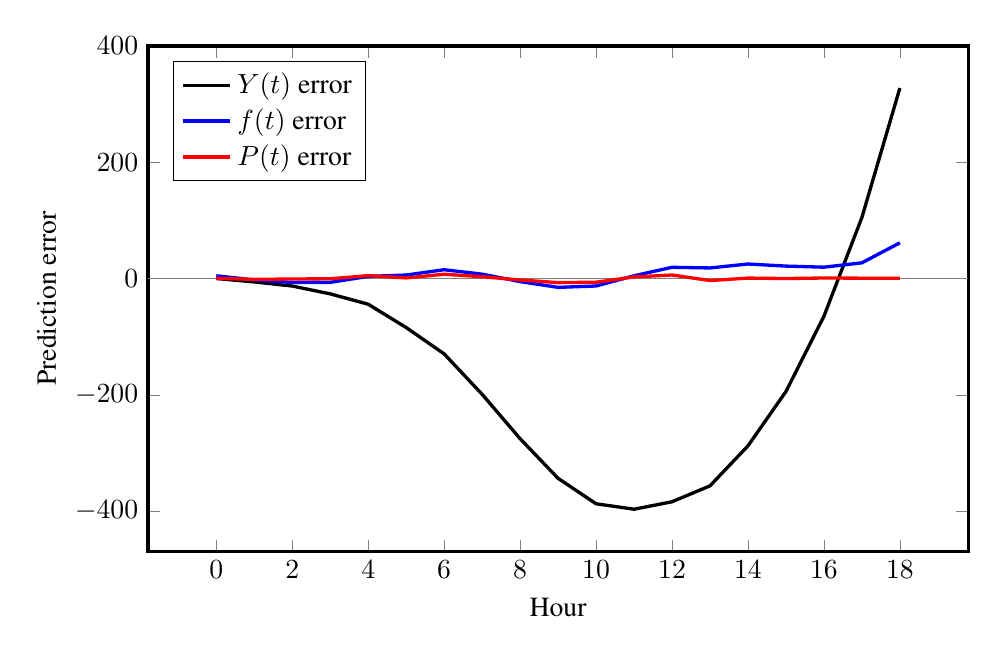
\begin{tikzpicture}
\tikzset{%%
  every mark/.append style={scale=1.0},%%
  scale=1.0%%
}
\pgfplotsset{%%
  every axis/.append style={font=\normalsize}%%
}
%%
\begin{axis}[%%
  axis line style=very thick,%%
  enlargelimits=true,%%
  height=8cm,%%
  legend cell align=left,%%
  legend pos=north west,%%
  plotStyle/.style={very thick,mark=none},%%
  width=12cm,%%
  %% x axis
  xlabel={\normalsize Hour},%%
  %% y axis
  ylabel={\normalsize Prediction error},%%
  scaled y ticks=false,%%
  y tick label style=/pgf/number format/fixed%%
]
%%
%%
%% Horizontal line through origin.
\draw[gray,thin] ({rel axis cs:0,0}|-{axis cs:0,0}) -- ({rel axis cs:1,0}|-{axis cs:1,0});
%%
%%
%% The errors from the function Y(t).
\addplot[plotStyle,black] coordinates {
  (0, 0)
  (1, -5.88048)
  (2, -12.932866976)
  (3, -26.4139500068512)
  (4, -44.2090871238634)
  (5, -84.3112260121421)
  (6, -129.593763091908)
  (7, -199.075431312002)
  (8, -275.374875488336)
  (9, -343.551886419261)
  (10, -387.231375460598)
  (11, -396.605020433375)
  (12, -383.804024934658)
  (13, -356.434507057967)
  (14, -287.664541780891)
  (15, -194.248657701939)
  (16, -64.871418468999)
  (17, 105.013675926656)
  (18, 327.380712546315)
};
\addlegendentry{$Y(t)$ error}
%%
%%
%% The errors from the function f(t).
\addplot[plotStyle,blue] coordinates {
  (0, 4.6567)
  (1, -2.4752)
  (2, -6.8447)
  (3, -6.6216)
  (4, 3.6067)
  (5, 5.9592)
  (6, 15.0853)
  (7, 7.48879999999997)
  (8, -5.34809999999999)
  (9, -15.2407999999999)
  (10, -12.8783)
  (11, 4.70079999999984)
  (12, 19.2323)
  (13, 18.1504000000001)
  (14, 24.9116999999994)
  (15, 21.3191999999997)
  (16, 19.4463000000005)
  (17, 26.9608000000006)
  (18, 61.3489000000011)
};
\addlegendentry{$f(t)$ error}
%%
%%
%% The errors from the function P(t).
\addplot[plotStyle,red] coordinates {
  (0, 0.325908374101179)
  (1, -1.520941396282)
  (2, -0.839570799353563)
  (3, -0.494371877829558)
  (4, 4.90624990862652)
  (5, 1.01747487421973)
  (6, 7.32201420820374)
  (7, 3.03346351836217)
  (8, -2.51764419720018)
  (9, -7.10958654485057)
  (10, -6.3621623067657)
  (11, 2.65874195265269)
  (12, 6.00818421689519)
  (13, -3.54301118206945)
  (14, 0.713399396664727)
  (15, -0.052826479318696)
  (16, 0.860664750116371)
  (17, 0.551981409786777)
  (18, 0.353479499997434)
};
\addlegendentry{$P(t)$ error}
\end{axis}
\end{tikzpicture}

\end{document}
